\documentclass[conference]{IEEEtran}
\usepackage{standalone}
\usepackage{times}
\usepackage{float}

%% Additional packages
\usepackage{times}
\usepackage{amsmath}
\usepackage{amsthm}
\usepackage{amssymb}
\usepackage{amsfonts}
\usepackage{mathtools}
%\usepackage{calc}
\usepackage{subfigure}
\usepackage{graphicx}
\usepackage{color}
\usepackage{url}
%\usepackage{lineno}
%\usepackage{ulem} % for underlining and strike through
%\normalem % reset emph to normal
%\usepackage{setspace} % for line spacing - e.g. 1.5, 2
\usepackage[usenames,x11names]{xcolor}
%\usepackage{xspace} % for inserting a space in TeX commands if needed
%\usepackage{caption}
\usepackage[bookmarks=true]{hyperref}
%\renewcommand{\thesubfigure}{\relax} % no subfig counters
%\let\chapter\section % algorithm2e natbib compatibility
%\usepackage{accents}
%\usepackage[titletoc,toc,title]{appendix}
%\usepackage{longtable}
%\usepackage{setspace}
\usepackage{multicol}

%% Packages
%\usepackage[margin=1in]{geometry}
%\usepackage[abs]{overpic}
\usepackage[linesnumbered,vlined,ruled]{algorithm2e}
%\usepackage{multirow} % for cell tables spanning multiple rows
\usepackage{tikz,pgf}%,tikz-3dplot}
\usetikzlibrary{arrows,automata,shapes,calc,backgrounds,spy,positioning}
%\usetikzlibrary{external}
%\tikzexternalize
%\usepackage[numbers]{natbib}
%\usepackage[sort,round]{natbib}
%\usepackage{lipsum}
\usepackage{epstopdf}

\theoremstyle{plain}
\newtheorem{theorem}{Theorem}
\newtheorem{cor}{Corollary}
\newtheorem{prop}{Proposition}
\newtheorem{lemma}{Lemma}

\theoremstyle{definition}
%\newtheorem{definition}{Definition}
\newtheorem{remark}{Remark}
\newtheorem{cond}{Condition}

\newtheorem{example}{Example}
\newtheorem{problem}{Problem}
%\newtheorem{assumption}{Assumption}


%%% figure path
\graphicspath{{figures/}}

%% Remove footnote mark
%\renewcommand{\footnotemark}{}

%%% Redefine qed symbol
%\renewcommand{\qedsymbol}{$\blacksquare$}

%% Projection symbol
%\newcommand{\project}[1]{\! \upharpoonright_{#1}}


%% Theorems 
%\newtheorem{theorem}{Theorem}[section]
%\newtheorem{proposition}[theorem]{Proposition}
%\newtheorem{corollary}[theorem]{Corollary}
\newtheorem{definition}[theorem]{Definition}
%\newtheorem{lemma}[theorem]{Lemma}
%\newtheorem{remark}[theorem]{Remark}
%\newtheorem{remarks}[theorem]{Remarks}
%\newtheorem{example}[theorem]{Example}
%\newtheorem{algo}[theorem]{Algorithm}
%\newtheorem{problem}[theorem]{Problem}
%\newtheorem{Procedure}[theorem]{Procedure}
%\newcommand{\exampler}[2]{\medskip \hskip -\parindent {\bf Example #1 Revisited.~}{\it #2}\medskip}

%% Percent
%\newcommand\oprocendsymbol{\hbox{$\square$}}
%\newcommand\oprocend{\relax\ifmmode\else\unskip\hfill\fi\oprocendsymbol}
%\def\eqoprocend{\tag*{$\bullet$}}

%% Enumerate environment
%\renewcommand{\labelenumi}{(\roman{enumi})}
%\renewcommand{\labelenumii}{(\alph{enumii})}

%% Breakable comma
%\mathchardef\breakingcomma\mathcode`\,
%{\catcode`,=\active
%  \gdef,{\breakingcomma\discretionary{}{}{}}
%}
%\newcommand{\breqn}[1]{\mathcode`\,=\string"8000 #1}

%% Other Stuff
%\newcommand{\margin}[1]{\marginpar{\tiny\color{blue} #1}}
%%\addtolength{\marginparwidth}{-0.3in}
\newcommand{\todo}[1]{\vskip 0.05in \colorbox{yellow}{$\Box$ \ttfamily\bfseries\small#1}\vskip 0.05in}
%\newcommand{\todo}[1]{}
%\newcommand{\vers}{\operatorname{vers}}

%% Roman, calligraphic, boldface, double barred letters
\newcommand{\RM}[1]{\mathrm{#1}}
\newcommand{\CA}[1]{\mathcal{#1}}
\newcommand{\BF}[1]{\mathbf{#1}}
\newcommand{\IT}[1]{\mathit{#1}}
\newcommand{\BB}[1]{\mathbb{#1}}
\newcommand{\TT}[1]{\mathtt{#1}}
\newcommand{\FK}[1]{\mathfrak{#1}}
\newcommand{\BS}[1]{\boldsymbol{#1}}

%%% Temporal logic symbols
\newcommand{\notltl}{\neg}
\newcommand{\andltl}{\wedge}
\newcommand{\orltl}{\vee}
\newcommand{\Next}{\ensuremath{\bigcirc}}
\newcommand{\Always}{\ensuremath{\ \square\ }}
\newcommand{\Event}{\ensuremath{\ \diamondsuit\ }}
\newcommand{\Until}{\ \CA{U}\ }
\newcommand{\Implies}{\Rightarrow}
\newcommand{\Equiv}{\Leftrightarrow}
%\newcommand{\Not}{\lnot}
\newcommand{\True}{\top}
\newcommand{\False}{\perp}
%\def\prop{\TT{data}}
%\def\popt{\pi}
\newcommand{\AP}{AP}
\newcommand{\pred}{\xi}

\newcommand{\Real}{\BB{R}}

%% Abbreviations
%\def\eg{e.g.\xspace}
%\def\Eg{E.g.\xspace}
%\def\ie{i.e.\xspace}
%\def\Ie{I.e.\xspace}
%\def\etc{etc.\xspace}
%\def\vs{vs.\xspace}
%\def\wrt{w.r.t.\xspace}
%\def\etal{et al.\xspace}

%% Exotic words
\newcommand{\buchi}{B\"uchi\ }

%% Symbols of automata
\newcommand{\PA}{\mathcal{P}}
\newcommand{\BA}{\mathcal{B}}
%\newcommand{\FA}{\mathcal{F}}

\newcommand{\TS}{\mathcal{F}}
\newcommand{\LA}{\mathcal{L}}
\newcommand{\KA}{\mathcal{K}}
\newcommand{\MDP}{\mathcal{M}}
\newcommand{\RA}{\mathcal{R}}
\newcommand{\FSA}{\mathcal{A}}

\newcommand{\TSX}{\BB{V}_\TS}
\newcommand{\TSE}{\BB{E}_\TS}
\newcommand{\TSEE}{\BB{E}}

\newcommand{\DTL}{DTL\xspace}


%% Short macros for arrows
\newcommand{\la}{\leftarrow}
\newcommand{\ra}{\rightarrow}
\newcommand{\ras}[1]{\stackrel{#1}{\rightarrow}}
\newcommand{\asgn}{\la}
\newcommand{\proj}[2]{{#1}{\downharpoonright_{#2}}}

\newcommand{\df}{\xspace\RM{d}}

%% Names of the Algorithms
%\newcommand{\optrun}{\textsc{Optimal-Run}\ }
%\newcommand{\exactmultioptrun}{\textsc{Exact-Multi-Robot-Optimal-Run}\ }
%\newcommand{\constR}{\textsc{Construct-Region-Automaton}\ }
%\newcommand{\constT}{\textsc{Construct-Team-TS}\ }
%\newcommand{\syncT}{\textsc{Sync-Team-TS}\ }
%\newcommand{\boundOpt}{\textsc{Bound-Optimality}\ }

% Custom operators
%\DeclareMathOperator*{\argmin}{arg\,min}
\newcommand{\norm}[1]{\left\| {#1} \right\|}
\newcommand{\norminf}[1]{\left\| {#1} \right\|_{\infty}}
\newcommand{\normeucl}[1]{\left\| {#1} \right\|_{2}}
\newcommand{\abs}[1]{\left| {#1} \right|}
\newcommand{\card}[1]{\left| {#1} \right|}
\newcommand{\spow}[1]{2^{#1}}
%\newcommand{\interior}[1]{\accentset{\smash{\raisebox{-0.12ex}{$\scriptstyle\circ$}}}{#1}\rule{0pt}{2.3ex}}
\newcommand{\interior}[1]{\mathring{#1}}
\DeclareMathOperator{\diag}{diag}
\newcommand{\lift}{\upharpoonright}
%
%% Display a grid to help align images
%\beamertemplategridbackground[1cm]
%\usepackage[style=numeric-comp]{biblatex}
\usepackage{cite}


%\documentclass[letterpaper, 11pt, onecolumn]{TemplateFiles/ieeeconf}
%\IEEEoverridecommandlockouts \overrideIEEEmargins 
%\pagestyle{plain}

%\usepackage[ruled,vlined,linesnumbered,boxruled]{algorithm2e}
%\usepackage{mathrsfs}
%\usepackage{graphicx}
%\usepackage{amsfonts}
%\usepackage{amsmath}
%\usepackage{amssymb}
%\usepackage{array}
%\usepackage{flafter}
%\usepackage{tabu}
%\usepackage{cite}
%\usepackage{subfigure}
%\usepackage{verbatim}
%\usepackage{bbm}
%\usepackage[usenames]{color}
%\usepackage[svgnames]{xcolor}

%\usepackage{balance}

%\usepackage{nicefrac}
%\usepackage{psfrag}
%\usepackage{umoline}
%\usepackage{hyperref}
%\usepackage{appendix} %[2009/09/02 v1.2b extra appendix facilities]
%\let\proof\relax
%\let\endproof\relax
%\usepackage{amsthm}	% This is needed for \newtheorem and proof environment.
% \usepackage{natbib} % for citing the papers with auther-year format in parantheses.
%\usepackage[numbers, sort]{natbib}

%\usepackage{etoolbox}

%\providecommand{\citet}[1]{\citeauthor{#1}\,[\citeyear{#1}]}
%\providecommand{\citep}[1]{\cite{#1}}

%\newtheorem{thm}{Theorem}
%\newtheorem{Def}{Definition}
%\newtheorem{Problem}{Problem}
%\newtheorem{Lem}{Lemma}
%\newtheorem{Cor}{Corollary}
%\newtheorem{assumption}{Assumption}
%\newtheorem{proposition}{Proposition}
%\newtheorem{definition}{Definition}
%\newtheorem{property}{Property}
%\newtheorem{Remark}{Remark}
%\newtheorem{exmp}{Example}[section]
%\newenvironment{proof}[1][Proof]{\begin{trivlist}
%\item[\hskip \labelsep {\bfseries #1}]}{\end{trivlist}}

%\newcommand{\TypeOfDoc}{IJRR} % This either can be TR or Conf or IJRR
%\newcommand{\FinalFlag}{No} % This either can be No or Accepted
%\newtoggle{finalpaper}
%\toggletrue{finalpaper}
%\togglefalse{finalpaper}

\graphicspath{{./figs/}}

%\allowdisplaybreaks[1]

%\newcommand{\kXX}[1]{\color{blue} XX #1 XX \color{black}}
%newcommand{\AXX}[1]{\color{purple} XX #1 XX \color{black}}
\newcommand{\aXX}[1]{\color{orange} #1  \color{black}}
\newcommand{\axx}[1]{\aXX{#1}}


\newcommand{\pr}[1]{\textbf{#1:} }

\newcommand{\codeline}[1]{\par{\ttfamily #1 \par}}  % This line is added because sth like this \newcommand{\initeali}{\verb|InitializeEdge|} does not work. For further details please check out this link % http://tex.stackexchange.com/questions/86071/newcommand-for-verbatim
% please do not delete above comments as it can be really confsing


%%%%%%%%%%%%%%%% symbols
\newcommand{\tv}{\varpi} % tube volume (edge tube volume)
\newcommand{\td}{\Gamma} % tube distance (edge tube distance)

%%%%%%%%%%%%%%%%%%%%%%%%%%%%%%%%%%%%%%%%%%%%%%%%%% To reduce pages
%\textfloatsep = 0pt
%\renewcommand{\baselinestretch}{0.96}
%%%%%%%%%%%%%%%%% Make bibs smaller
%\renewcommand{\IEEEbibitemsep}{0pt plus 2pt}
%\makeatletter
%\IEEEtriggercmd{\reset@font\normalfont\footnotesize}
%\makeatother
%\IEEEtriggeratref{1}

%%%%%%%%%%%%%%%%% margins
%\usepackage{geometry}
% \newcommand{\papermargin}{0.97in} % IEEE asks for 0.75 on all pages, but the first page
% %\newgeometry{top=0.75in,bottom=.75in,right=.75in,left=.75in}
% \newgeometry{top=\papermargin,bottom=\papermargin,right=\papermargin,left=\papermargin}
% \newgeometry{top=1.in,bottom=1.in,right=1.in,left=1.in}

\let\labelindent\relax
\usepackage{enumitem}


% numbers option provides compact numerical references in the text. 

% Table caption wrangling
\usepackage{etoolbox}
\makeatletter
\patchcmd{\@makecaption}
  {\scshape}
  {}
  {}
  {}
\makeatletter
\patchcmd{\@makecaption}
  {\\}
  {.\ }
  {}
  {}
\makeatother

\newcommand{\Ali}[1]{{\color{green} Ali: #1}}
\newcommand{\cristi}[1]{{\color{orange} Cristi: #1}}
%\newcommand{\rohan}[1]{{\color{blue} Rohan: #1}}
\allowdisplaybreaks[1]

\begin{document}

% paper title
\title{\huge Mobile Eye in the Sky: Copter-Rover Coordination for Space Exploration}

%\author{Takahiro Sasaki, Kyohei Otsu, Ali-akbar Agha-mohammadi, Kamak Ebadi}

\maketitle

\begin{abstract}
In this paper, we consider the problem of planetary exploration with a two-agent team composed of a Mars rover and copter. Images by a copter can help estimation or navigation of a rover. In such a mission, how a copter learns where to map for a rover is of great interest in a two-agent team. 
This paper answers this where to map by a copter while minimizing uncertainty of images from a rover’s camera.
\end{abstract}

\IEEEpeerreviewmaketitle
%%%%%%%%%%%%%%%%%%%%%%%%%%%%%%%%%%%%%%%%%%%%%%%%
%%%%%%%%%%%%%%%%%%%%%%%%%%%%%%%%%%%%%%%%%%%%%%%%

\section{Introduction}

%\subsection*{Related Work}
%\subsection*{Contributions}

\section{Problem Description}
This section gives a formal definition of the problem we are going to address. 

\pr{Problem}
A two-agent team composed of a Mars rover and copter is considered. This paper automates the process of where to map by a copter in order to minimize the covariance or the localization belief of a rover while considering the copter’s body path.
Copter’s constraints coming from a battery is described as follows:
\begin{itemize}
    \item Two flights per sol
    \item Two minutes per flight
\end{itemize}
 Figure~\ref{fig:8_1} shows a belief propagation of a rover and Fig.~\ref{fig:8_2} illustrates an image of where to map by a copter. The copter can take images within the limitation of the battery at one step of the rover.
 
\pr{Rover and Helicopter Description}
The rover and helicopter configurations are denoted by $x^r$ and $x^c$, respectively. The extended state $x=(x^r,~x^c)$ includes both.

\pr{Rover and Helicopter Measurements}
Let $z^r_k$ and $z^c_k$ the measurements (images) by the rover and the copter at the $k$-th time step, respectively. Sequences of observations are defined as
\begin{align}
    z^r_{0:k}&=\{z^r_0,z^r_1,\cdots,z^r_k\}\\
    z^c_{k,1:j}&=\{z^c_{k,1},z^c_{k,2},\cdots,z^c_{k,j}\}
\end{align}
where $0 \leq k \leq T$ and a copter takes $j$ images at the $k$-th rover step.

\pr{Map Belief}
We denote the map of the environment by $m$ and assume the environment is stationary. The knowledge we have about the environment is obtained via noisy sensors. Therefore, the best we can have is a probabilistic representation of $m$, i.e., the map belief
\begin{align}
    b^m=p(m|z, x)
\end{align}

\pr{Measurement Model}
The measurement model describes the probability distribution over all possible observations given the robots' state $x$ and the environment map $m$.
\begin{align}
    p(z|m, x)
\end{align}



\begin{figure}[h]
		\centering
		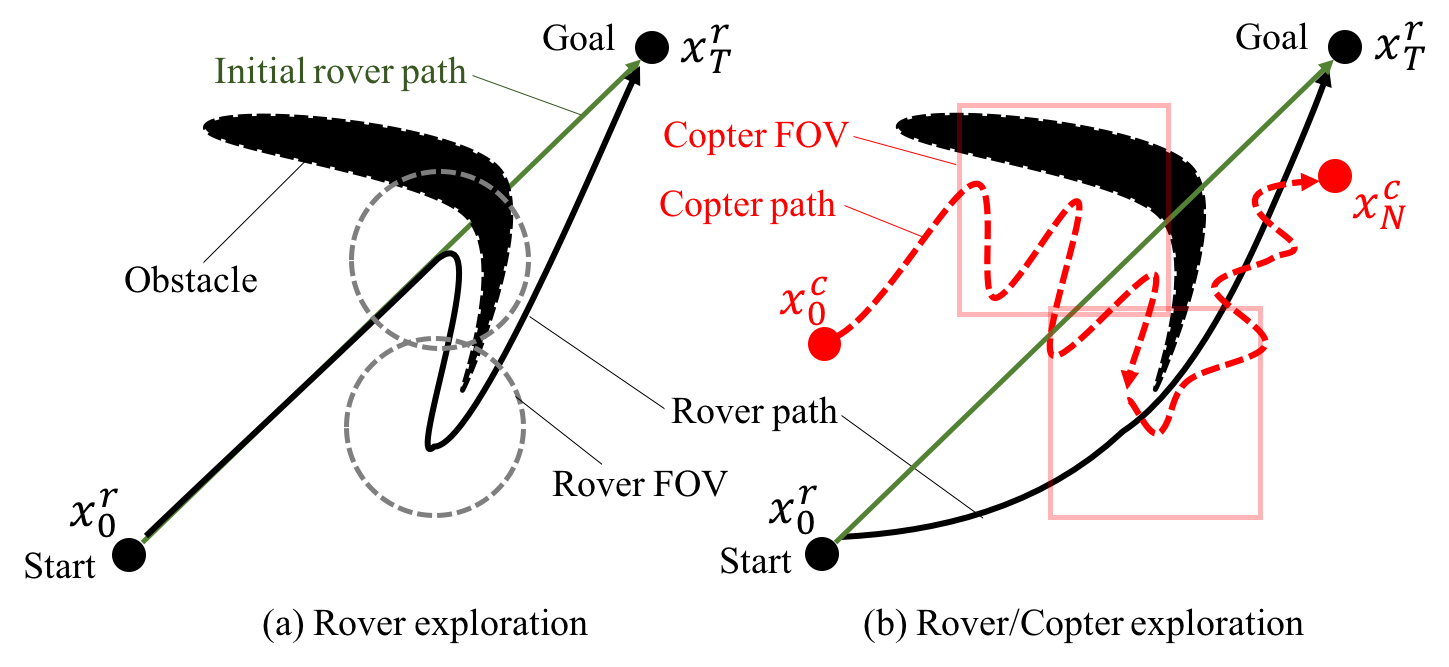
\includegraphics[width=1.0\columnwidth]{figs/8_1.png}
		\caption{Rover path.}
		\label{fig:8_1}
		\centering
		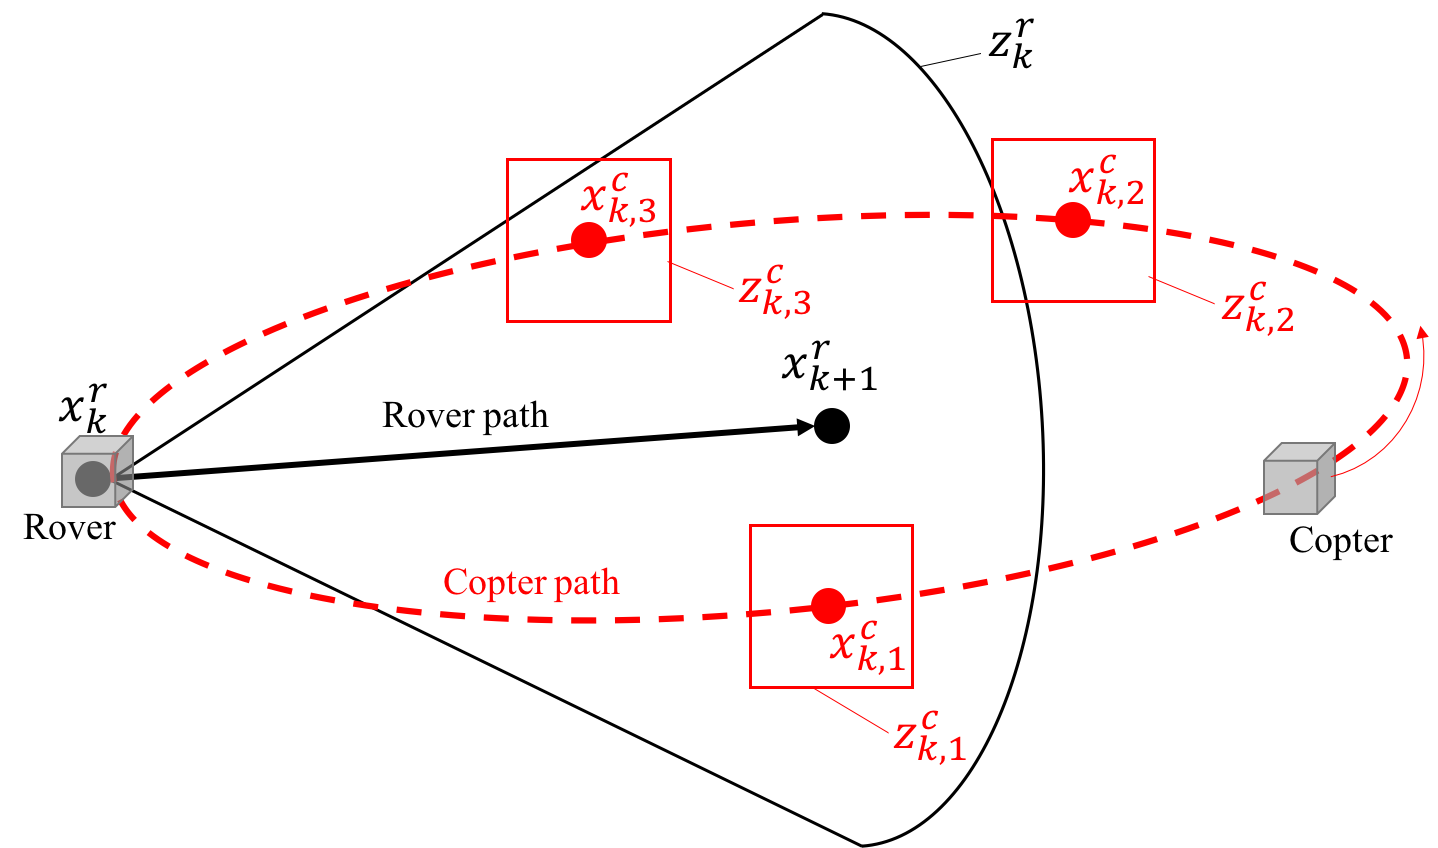
\includegraphics[width=1.0\columnwidth]{figs/8_2.png}
		\caption{Where to map.}
		\label{fig:8_2}
\end{figure}


\section{Mapping}

\pr{Map Representation}
We consider maps from both rover and copter and use a surf feature mapping. Vectors or matrices $m^r$ and $m^c$ denote maps by a rover and a copter, respectively. Finally, a map can be obtained by combining $m^r$ and $m^c$.

\pr{Map Update}
The map of a rover and a copter can be updated as follows:
\begin{align}
    m^r_{k+1}&=\tau^r_m (m_k, x^r_{k+1}, z^r_{k+1})\\
    m^c_{k+1}&=\tau^c_m (m_k, x^c_{k+1}, z^c_{k+1})
\end{align}
where
\begin{align}
    z^r_{k+1} &\sim p(\cdot |x^r_{k+1})\\
    x^r_{k+1} &\sim p(\cdot |x^r_k, u^r_k, w^r_k)\\
    z^c_{k+1} &\sim p(\cdot |x^c_{k+1})\\
    x^c_{k+1} &\sim p(\cdot |x^c_k, u^c_k, w^c_k).
\end{align}
Therefore, using these $m^r_{k+1}$ and $m^c_{k+1}$, the map at the $k$-th time step can be obtained by

\begin{eqnarray}
m_{k+1} =
  \begin{cases}
    \tau_m (m^r_{k+1}, m^c_{k+1}) & (k+1 = l)\\
    m^r_{k+1} & (k+1 \neq l)
  \end{cases}
\end{eqnarray}

%%%%%%%%%%%%%%%%%%%%%%%%%%%%%%%%%%%%%%%%%%%%%%%%%%%%%%%%%%
\section{Rover Localization}
This section considers belief update for a rover localization. Belief update of a map is given by
\begin{eqnarray}
    b^{m}_k=
    \begin{cases}
    p(m_k | z^r_{0:k}, x^r_{0:k}, z^c_{k,1:j}, x^c_{k,1:j}) & (k=l)\\
    p(m_k | z^r_{0:k}, x^r_{0:k}) & (k \neq l)
    \end{cases}
\end{eqnarray}
Belief update of a rover localization is given by
\begin{align}
    b^r_{k+1}=\tau^r (b^r_k, b^m_k, u^r_k, z^r_{k+1}; m_{k+1}).
\end{align}

\section{Planning: copter where to map}
\subsection{Planning Objective}
%Covariance (Exploitation)\\

We find a helicopter position that minimizes the following cost function:
\begin{align}
    &x^{c*}=\arg\min_{x^c \in X^c} \sum^T_{k=1} P^{r+}_k\label{eq:c1}\\
     &{\rm s.t.} \hspace{5mm} D^c_{\min}(x^c_{alt}) \leq D^c_k \leq D^c_{\max}(x^c_{alt})\label{eq:st1}\\
    &\hspace{10mm} \sum^{n}_{i=0} L^c_{k,i} \leq L^c_{\max}(t^c_{search}), ~~0\leq i \leq n \label{eq:st2}
\end{align}
where
\begin{align}
P^{r+}_k&={\rm Cov}(x^{r+}_k) = {\rm Cov}(x^{r}_k | z^r_{0:k})\label{eq:p1}\\
&={\rm VO}(z^r_0,~z^r_1,\cdots,~z^r_k)\simeq {\rm VO}(z^r_k).\label{eq:p2}
\end{align}
Note that Cov($\cdot$) and VO($\cdot$) denote the covariance and the visual odometry, respectively.

\subsection{Constraints}

\pr{Resolution constraint}
A resolution of an image from a copter depends on a camera performance and a altitude of a copter $x^c_{alt}$.
%\begin{align}
%    \zeta=k x^c_{alt}
%\end{align}

\pr{Field-of-view constraint}
Equation~\eqref{eq:st1} represents the constraint that the area of the image depends on the altitude of the copter.
A field-of-view (FOV) $D^c$ is determined by an altitude of a copter.
\begin{align}
    D^c_{\min}(x^c_{alt}) \leq D^c_k \leq D^c_{\max}(x^c_{alt})
\end{align}

\pr{Flight time constraint}
Equation~\eqref{eq:st2} represents the constraint that the searching range $L^c$ depends on the flight time $t^c_{search}$ coming from the battery limitation of the copter.
\begin{align}
    \sum^{n}_{i=0} L^c_{k,i} \leq L^c_{\max}(t^c_{search})
\end{align}
where $n$ is the number of the areas for searching by the copter.

\pr{Flight interval constraint}
``{\it When to map}'' is also an interesting problem.

%\textcolor[gray]{0.5}{
%\section{Planning: copter body path planning}
%\subsection{Planning Objective}
%Using the cost $C(b_k, u_k)$,
%\begin{align}
%    &u^{c*}_{0:k}=\arg\min_{x^c \in X^c} \mathbb{E} \sum^T_{k=0} C(b^r_k, u_k; m_k (u^c_{0:k}))\\
%    &{\rm s.t.} \hspace{5mm} ||u^c_{0:k}||< \delta\label{eq:st10}\\
%    &\hspace{10mm} x^r_T \in goal^r\label{eq:st20}
%\end{align}
%}
%Observation $z_k$ is given by
%\begin{align}
%z_k=x^r_k-L^m_k(x^c_k)
%\end{align}
%\textcolor[gray]{0.5}{
%\subsection{Constraints}
%\pr{Input constraint}
%Equation~\eqref{eq:st10} represents the constraint that %the limitation of the copter control input as follow:
%\begin{align}
%    ||u^c_{0:k}||< \delta
%\end{align}
%\pr{Position constraint}
%Equation~\eqref{eq:st20} represents the constraint that the rover need to reach the goal at the final step $T$.
%\begin{align}
%    x^r_T \in goal^r
%\end{align}
%}
\section{Search Method: copter where to map}
This section provides a process of a searching method for solving the cost function in the former section.
%\subsection{Grid the Search Space}
%First of all, we grid the searching space to determine where to map and the copter's path as in Fig.~\ref{fig:8_3}. These grid spaces are determined by a FOV of a copter.
%\begin{figure}[b]
%		\centering
%		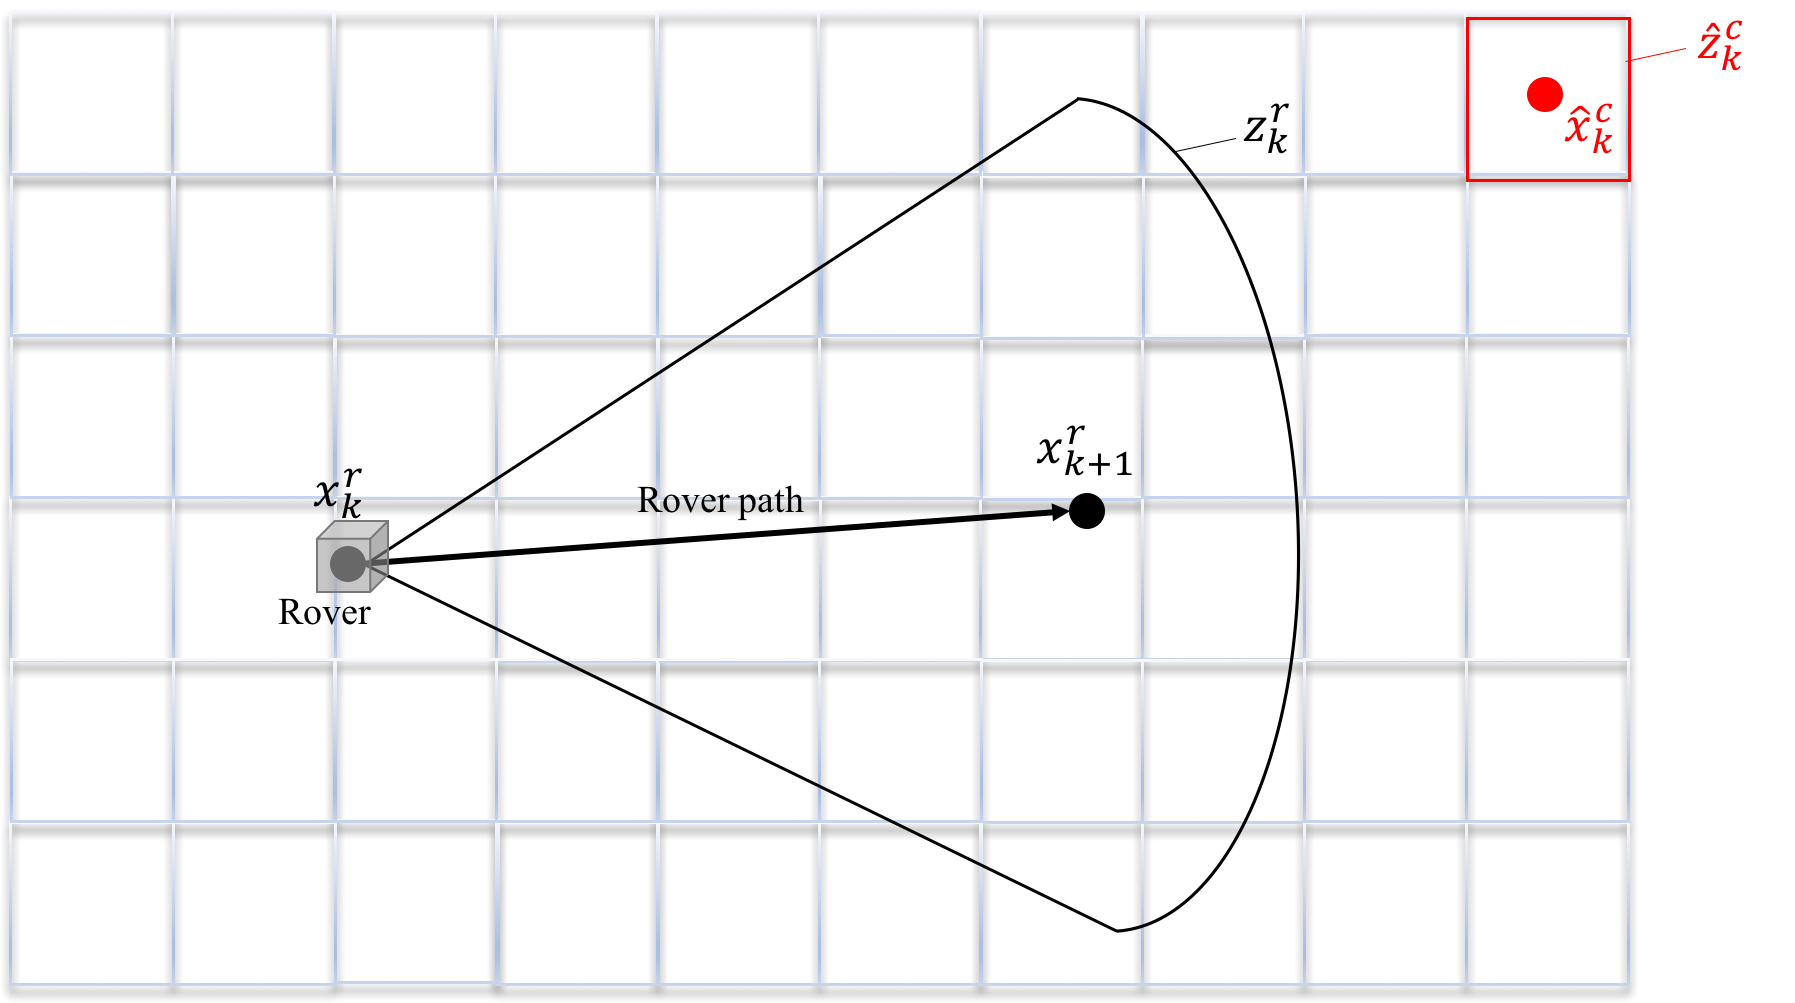
\includegraphics[width=1.0\columnwidth]{figs/8_3.png}
%		\caption{Searching space grid.}
%		\label{fig:8_3}
%\end{figure}
%\subsection{Planning Objective~2: Coverage (Exploration)}
\subsection{Perception Performance Prediction}
Our method investigates unseen or uncertainty areas by a copter. 
Here, we consider the performance of the VO system as the evaluating measurement of the rover localization belief $b^r_{k+1}$. We know how to predict the most likely future measurement $\{ \grave{z}^r_t \}$ for all $t>k$ in Ref.~\cite{IEEE:Kyon}. We run a given VO algorithm on these synthetic images
\begin{align}
    {\rm VO}: (\grave{z}^r_i,\grave{z}^r_{i+1}) \to (\Delta \grae{x}_{i,i+1},\Omega_{i,i+1}),\quad i=k,\cdots,t
\end{align}
where $\Delta \grave{x}_{i,i+1}$ denotes the displacement between two synthetic images $i$ and $i+1$ computed by VO, and $\Omega_{i,i+1}$ is the performance indicator for VO between time-steps $i$ and $i+1$, which includes Cov($x^{r}_{k+1} | z_{0:k+1}$) in Eq.~\eqref{eq:p1}. To evaluate the $k+1$-th Cov($x^{r}_{k+1} | z_{0:k+1}$), ``where to map'' by a copter can be obtained as shown the red areas in Fig.~\ref{fig:8_4}.

%\subsection*{Coverage (Exploration)}
%\begin{itemize}
%    \item Occluded area (using Viewshed analysis)
 %   \item Beyond rover’s perception horizon
%\end{itemize}

\subsection{Search the optimal path}
From the obtained the areas to map, next we search the optimal path (shortest path) using a traveling salesman problem (TSP).
%or a dynamic programming (DP).  
%\begin{figure}[h]
%		\centering
%		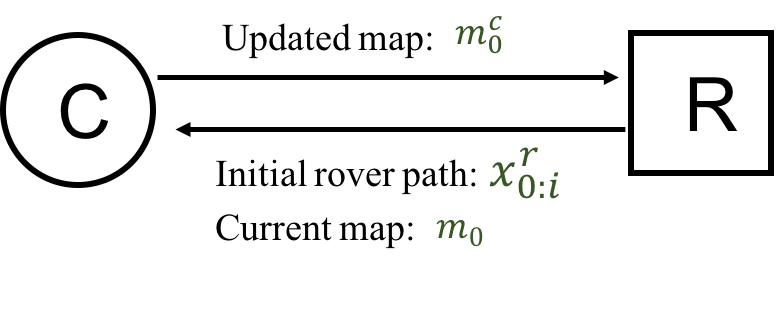
\includegraphics[width=1.0\columnwidth]{figs/8_4.png}
%		\caption{Creating the path (in the case of $n=3$).}
%		\label{fig:8_4}
%\end{figure}
\begin{figure}[h]
		\centering
		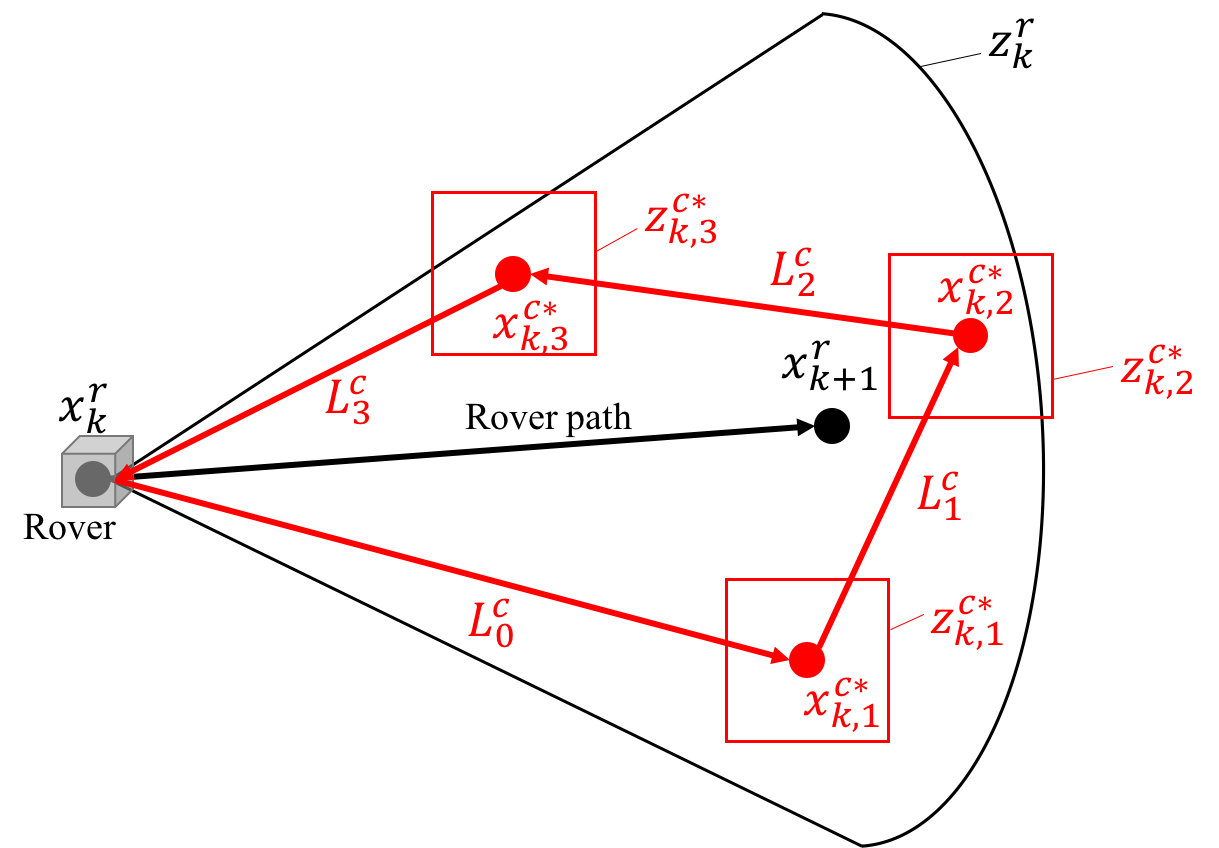
\includegraphics[width=1.0\columnwidth]{figs/8_10.png}
		\caption{Creating the path (in the case of $n=3$).}
		\label{fig:8_10}
\end{figure}

\section{Search Method: copter path planning}
\subsection{Informed RRT^*}





As a exploration, we search the occluded area by using viewshed analysis with $(x^r_k,~m_k)$. As a simple example of viewshed analysis, the coverage can be obtained as shown in Fig.~\ref{fig:vs}.



\begin{figure}[h]
		\centering
		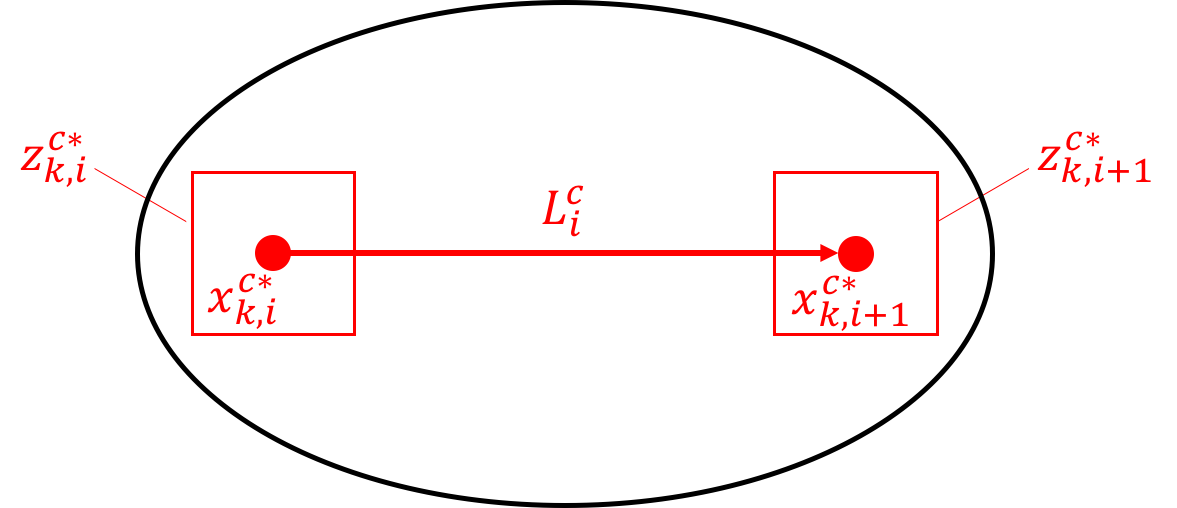
\includegraphics[width=1.0\columnwidth]{figs/8_11.png}
		\caption{Informed RRT^*.}
		\label{fig:8_11}
		\centering
		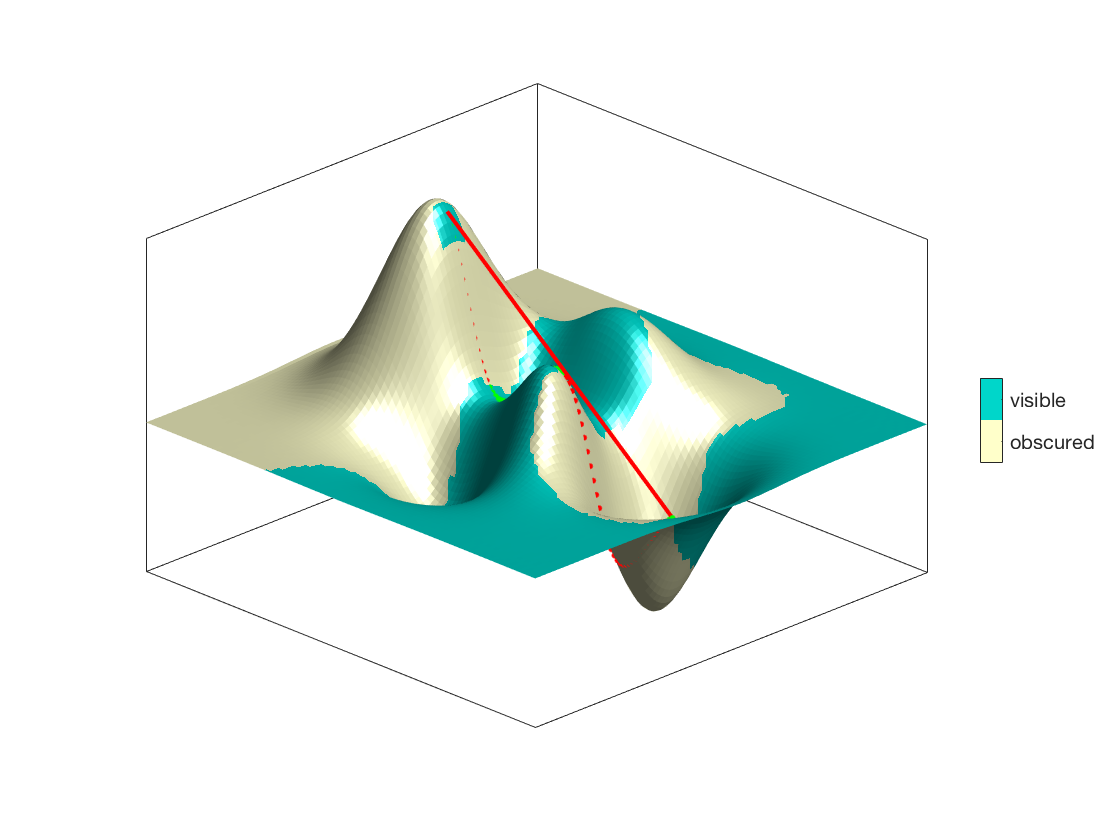
\includegraphics[width=1.0\columnwidth]{figs/vs.png}
		\caption{Viewshed analysis (example).}
		\label{fig:vs}
\end{figure}






\section{Simulation Results}

\section{Conclusion}

\begin{thebibliography}{1}

\bibitem{IEEE:Kyon}
K. Otsu, A. Agha-mohammadi, and M. Paton, ``Where to look? Predictive Perception with Applications to Planetary Exploration,'' in {\it IEEE Robotics and Automation Letters}, vol.xx, no.xx, pp.xx-xx, 201x.

\end{thebibliography}

\end{document}

